L'objectif de ce projet était la création d'un serveur\footnote{Un serveur au sens figuré du terme. Nous n'avons pas eu a faire de réseau, heureusement.}
sur lequel des joueurs (\textit{clients}) peuvent jouer au jeu des \textit{Amazones}. Il nous a aussi été demandé d'implémenter quelques clients même si cela était plutôt secondaire.

\subsection{Le jeu des Amazones}

Le jeu des amazons est un jeu de plateau où deux joueurs s'affrontent en jouant tour à tour.
Ils disposent chacun de reines\footnote{Plus exactement $\mathtt{floor}(4*(m/10 + 1))$ où $m$ est la largeur du plateau},
qui peuvent se déplacer comme des reines au jeu des échecs. Les reines doivent être espacés d'au moins 2 espaces ou d'un espace en diagonale.
Le jeu requiert que les reines soient symmétriques entre les joueurs et qu'il y ait autant de reines sur la ligne externe que sur les colonnes externes.

\begin{figure}[h!]
	\centering
	\newchessgame[
		setwhite={qb1, qg1, qa2, qh2},
		addblack={qb8, qg8, qa7, qh7}
	]
	\chessboard[showmover=false]
	\caption{Un jeu des Amazones.}
	\label{fig:amazon-game}
\end{figure}

Chaque joueur joue une reine puis tire une flêche depuis la position atteinte par la reine.
Les flêches agissent comme une reine dans le jeu des échecs mais ne peuvent traverser de reines ou d'autres flêches.
Le premier joueur qui ne peut pas jouer un coup valide perd.
\medbreak
Pour répondre à ce besoin, nous avons suivis les spécifications du sujet,
mis en place une infrastructure client-serveur, et réalisé plusieurs clients 
capable de jouer une partie, et souvent la gagner.

\subsection{Spécifications du sujet}
Le sujet nous demandait d'implémenter un modèle client-serveur et nous a
contraint à utiliser la librairie GSL.

\subsubsection{Structure Client Serveur}

La structure client-serveur, autrement appelée "monolithe", permet de séparer
la responsabilité des joueurs et du jeu en lui même. Le serveur représente le jeu. Il organise le
déroulement du jeu, retransmet l'information d'un client $x$ aux autres clients et vérifie que tout coup joué est valide.

\subsubsection{Utilisation de GSL}

Il nous a été demandé de représenter le plateau de jeu comme un graphe.
Cela permet quelques folies pour implémenter moultes plateaux intéressant.
Dans les règles des échecs, une case aura au plus 8 voisins, cela veut dire que dans le graphe, un noeud aura au maximum 8 voisins, alors qu'un graphe fait au moins 25 noeuds.
Pour représenter ce graphe, il nous a été demandé de le représenter par sa matrice d'adjacence.
Plus exactement, on stocke la direction entre le sommet i et le sommet j dans la matrice d'adjacence comme montré dans la Figure \ref{fig:ex-matrice-adj}.
Pour stocker cette matrice, nous étions contraints d'utiliser la GNU Scientific Library (GSL).
Cette librairie permet le stockage et traitement de matrices optimisées autrement appelées \textit{matrices creuses}.
Il aurait peut-être été plus judicieux de stocker une liste d'adjacence directement, mais les matrices creuses sous format Compressed Sparse Row (CSR) peuvent s'apparenter à cela.

\begin{figure}[H]
	\centering
	\raisebox{-0.5\height}{
		\subfloat[][Un graphe 2x2]{
			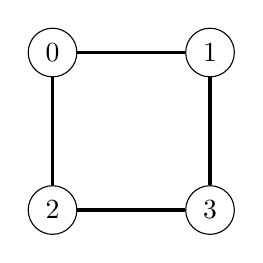
\begin{tikzpicture}
				\begin{scope}[every node/.style={draw, circle}]
					\node (0)[draw, circle] at (0,0) {0};
					\node (1)[draw, circle] at (2,0) {1};
					\node (2)[draw, circle] at (0,-2) {2};
					\node (3)[draw, circle] at (2,-2) {3};
				\end{scope}
				\begin{scope}[every edge/.style={draw, very thick}]
					\path [-] (0) edge node {} (1);
					\path [-] (0) edge node {} (2);
					\path [-] (1) edge node {} (3);
					\path [-] (2) edge node {} (3);

				\end{scope}
			\end{tikzpicture}
		}
	}
	\hspace{2em}
	\raisebox{-0.25\height}{
		\subfloat[][Sa matrice d'adjacence]{
			$\begin{bmatrix}
					NO\_DIR & EAST    & SOUTH   & NO\_DIR \\
					WEST    & NO\_DIR & NO\_DIR & SOUTH   \\
					NORTH   & NO\_DIR & NO\_DIR & EAST    \\
					NO\_DIR & NORTH   & WEST    & NO\_DIR \\
				\end{bmatrix}$
		}
	}
	\caption{Exemple de graphe et sa représentation en matrice d'adjacence}
	\label{fig:ex-matrice-adj}
\end{figure}

Enfin, le sujet demandait à implémenter les plateaux présenté en figure \ref{fig:all-boards}

\begin{figure}[H]
	\centering
	\subfloat[][Plateau classique]{
		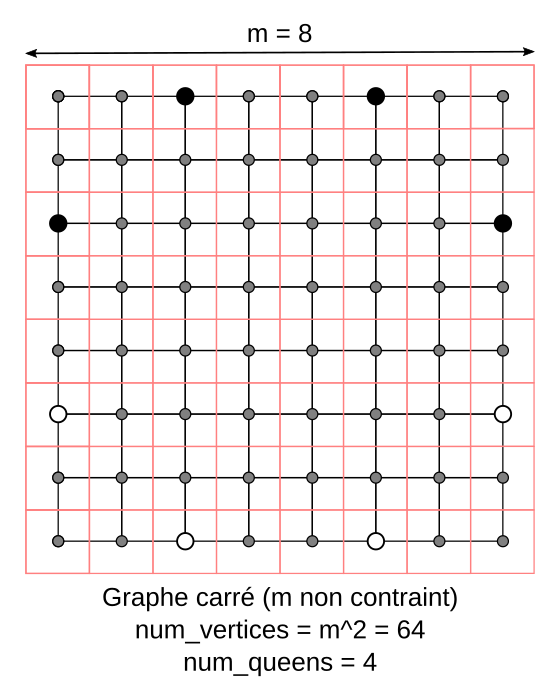
\includegraphics[width=0.3\linewidth]{classic_board}
	}
	\subfloat[][Plateau donut]{
		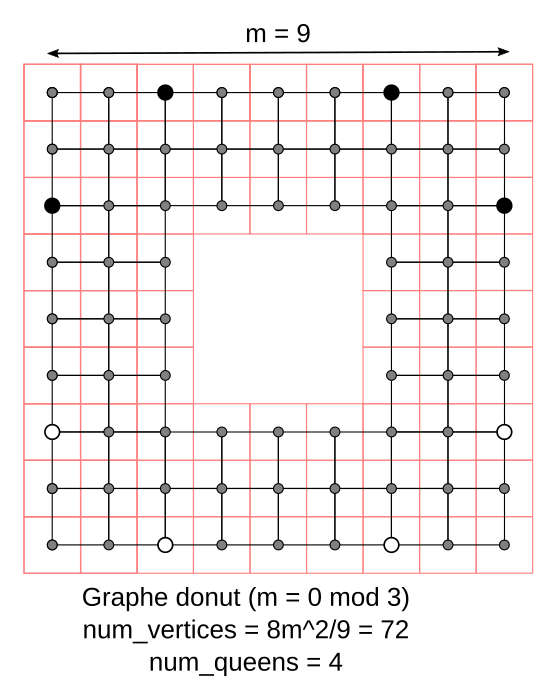
\includegraphics[width=0.3\linewidth]{donut_board}
	}

	\raisebox{-0.5\height}{
		\subfloat[][Plateau trèfle]{
			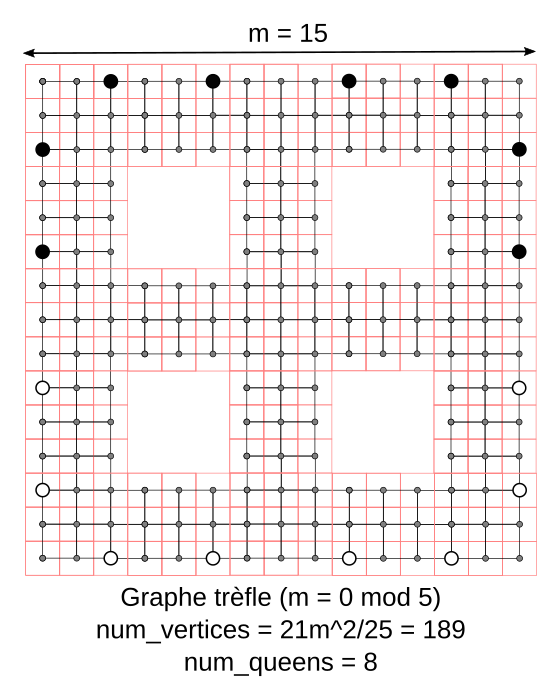
\includegraphics[width=0.3\linewidth]{clover_board}
		}
		\subfloat[][Plateau huit]{
			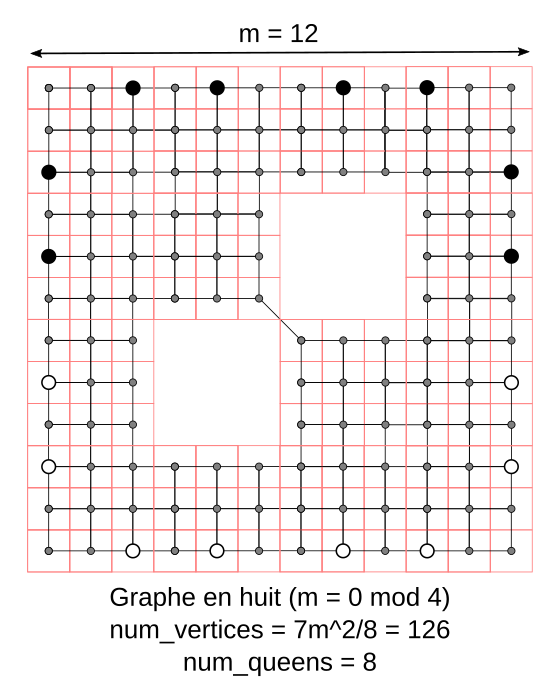
\includegraphics[width=0.3\linewidth]{eight_board}
		}
	}
	\caption{Les différents plateaux à implémenter et leurs graphes}
	\label{fig:all-boards}
\end{figure}

\subsubsection{Utilisation de libdl}

Chaque client devait être compilé en tant que librairie dynamique.
Le serveur devait lancer les clients en tant que librairies dynamiques ouvertes
au \textit{runtime} en utilisant la fonction \verb|dlopen| de la librairie \verb|libdl|